% ----------------------------
\chapter{Grundlagen der Codierungstheorie}
% ----------------------------

\begin{Beispiel}[Grundlagen der Codierungstheorie]
    Bei einem Satelliten, kann Rauschen durch thermische Störungen verursacht werden, während es bei Compact Discs durch Fingerabdrücke oder Kratzer entsteht. Wenn nun Binäre Daten über den Kanal übertragen werden und eine $0$ gesendet wird, sollte sie im Idealfall auch als eine $0$ empfangen werden, kann jedoch auch als $1$ oder unerkennbar empfangen werden. Anhand der empfangen Daten ist festzustellen, welche Nachricht gesendet wurde, hier liegt das Problem in der Kodierungstheorie.
    
    In \autoref{fig:kommunikationskanal} wird ein Kommunikationskanal dargestellt. 
    
    Eine Nachricht, mit \(x\) bezeichnet, soll am Ausgangspunkt übermittelt werden. Wenn die Nachricht in ursprünglicher Form über den Kanal übermittelt wird, würde Rauschen die Nachricht unkenntlich machen und die Information so verloren gehen.
    
    \begin{figure}[!ht]
        \centering
        {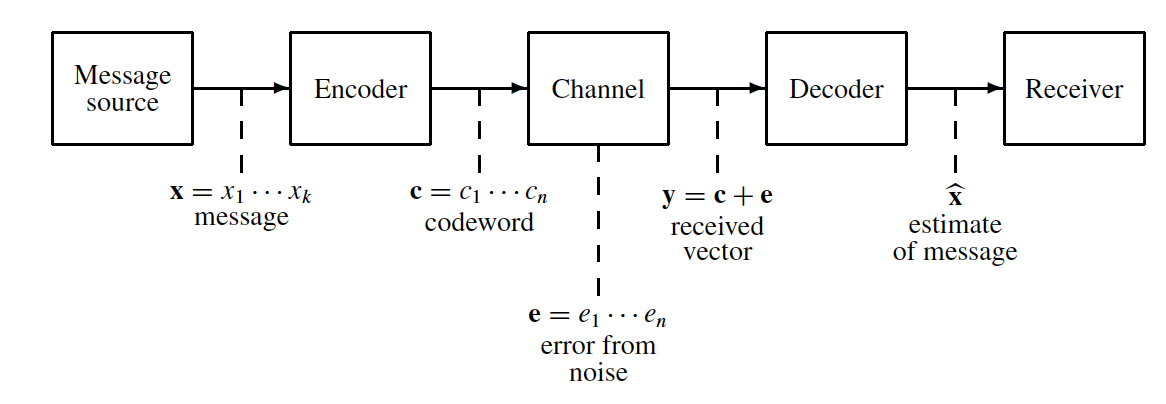
\includegraphics[width=0.7\textwidth]{./pic/LDPC-Codes1}}
        \caption{Kommunikationskanal}
        \label{fig:kommunikationskanal}
    \end{figure} 
    
    
    Die Kodierungstheorie beschäftigt sich damit, Informationen durch Ergänzung durch Redundanz so zu optimieren, dass sie den ursprünglichen Informationen gleichen. Dies geschieht indem der Kodierer die Information ergänzt, hier in der \autoref{fig:kommunikationskanal} als Codewort \(c\) benannt, und dann über einen Kanal übermittelt. Durch Rauschen, in der \autoref{fig:kommunikationskanal} als FehlerVektor \(e\) benannt, wird das Codewort verzerrt und man empfängt Vektor \(y\).
    
    
    Generell entspringen Codewort-Symbole aus einem Körper $\mathbb{F}_q$ mit \(q\) Elementen. Nachrichten und Codewörter sind Vektoren in den Vektorräumen $\mathbb{F}_{q}^{k}$ beziehungsweise $\mathbb{F}_{q}^{n}$.
    
    In \autoref{fig:kommunikationskanal} wird der FehlerVektor als \(e\) bezeichnet, dieser ist in der Abbildung die Differenz \( y - c \) aus dem Codewort \(c\), dass den Kanal betritt und dem empfangenden Vektor \(y\), der den Kanal verlässt. Die Abweichung zwischen dem Codewort \(c\)
    und dem Vektor \(y\) wird also durch den FehlerVektor \(e\) dargestellt. \cite[S. 2]{huffman}.
\end{Beispiel} 
    
    
    
\begin{definition}[Körper]
    Ein Körper ist eine algebraische Struktur. Diese besteht aus einer Menge und zwei Operationen die normalerweise als Mulitplikation mit $*$
    bezeichnet und als Addition mit $+$ bezeichnet benannt werden und bestimmte Axiome erfüllen. 
    Es gibt drei Körperer die man in der Untersuchung von linearen Codes sehr oft vorfindet. Diese sind das binäre Körper, mit zwei Elementen, das ternäre Körper mit drei Elementen und das quaternäre Körper mit vier Elementen. 
    
    \newpage
    Der Binärekörper $\mathbb{F}_2$ mit zwei Elementen \( \{0, 1\} \) hat die folgenden Additions- und Multiplikationstabellen
    
    \begin{table}[!h]
        \begin{center}
            \caption{Binärekörper $\mathbb{F}_2$}
            \label{tab:binäre Körper}
        \begin{tabular}{c|cc}
            
            $+$ & 0 & 1 \\
            \hline
            0 & 0 & 1 \\
            
            1 & 1 & 0 \\
            
            \end{tabular}
        \end{center}
        \end{table}
    
    \hfill
    
    \begin{table}[!h]
        \begin{center}
            \caption{Binärekörper $\mathbb{F}_2$}
            \label{tab:binäre Körper2}
            \begin{tabular}{c|cc}
                
                $*$& 0 & 1 \\
                \hline
                0 & 0 & 0 \\
                
                1 & 0 & 1 \\
                
                \end{tabular}
        \end{center}
        \end{table}
    \FloatBarrier
    Das ist auch der Ring der ganzen Zahlen Modulo 2. \\
    
    Der Ternärekörper $\mathbb{F}_3$ mit drei Elementen \( \{0, 1, 2\} \) hat Additions- und Multiplikationstabellen, die durch Addition und Multiplikation modulo 3 gegeben sind:
    
    
    \begin{table}[!h]
      \begin{center}
        \caption{Ternärekörper $\mathbb{F}_3$}
        \label{tab:ternäre Körper3}
        \begin{tabular}{c|ccc}
        
        $+$ & 0 & 1 & 2 \\
        \hline
        0 & 0 & 1 & 2 \\
        
        1 & 1 & 2 & 0 \\
        
        2 & 2 & 0 & 1 \\
        
        \end{tabular}
        \end{center}
    \end{table}
    
    \hfill
        \begin{table}[!h]
            \begin{center}
                \caption{Ternärekörper $\mathbb{F}_3$}
                \label{tab:ternäre Körper4}
                \begin{tabular}{c|ccc}
                
            $*$& 0 & 1 & 2 \\
            \hline
            0 & 0 & 0 & 0 \\
            
            1 & 0 & 1 & 2 \\
            
            2 & 0 & 2 & 1 \\
            
        \end{tabular}
    \end{center}
    \end{table}
    
    Der Quaternärekörper $\mathbb{F}_4$ mit vier Elementen \( \{0, 1, $\( \omega \)$, $\( \bar\omega\)$\} \) ist etwas komplizierter:\\ Er hat die folgenden Additions- und Multiplikationstabellen.\\
    $\mathbb{F}_4$ ist nicht der Ring der ganzen Zahlen, Modulo $4$:
    
    
    \begin{table}[!h]
        \begin{center}
          \caption{Quaternärekörper $\mathbb{F}_4$}
          \label{tab:quaternäre Körper5}
          \begin{tabular}{c|cccc}
            $+$ & 0 & 1 & $\omega$ & $\bar\omega$ \\
            \hline
            0 & 0 & 1 & $\omega$ & $\bar\omega$ \\
            1 & 1 & 0 & $\bar\omega$ & $\omega$ \\
            $\omega$ & $\omega$ & $\bar\omega$ & 0 & 1 \\
            $\bar\omega$ & $\bar\omega$ & $\omega$ & 1 & 0 \\
          \end{tabular}
          \end{center}
      \end{table}
    
    
    \hfill
    
        \begin{table}[!h]
        \begin{center}
            \caption{Quaternärekörper $\mathbb{F}_4$}
                \label{tab:quaternäre Körper6}
            \begin{tabular}{c|cccc}
            $*$ & 0 & 1 & $\omega$ & $\bar\omega$ \\
            \hline
            0 & 0 & 0 & 0 & 0 \\
            1 & 0 & 1 & $\omega$ & $\bar\omega$ \\
            $\omega$& 0 & $\omega$ & $\bar\omega$ & 1 \\
            $\bar\omega$& 0 & $\bar\omega$& 1 & $\omega$ \\
            \end{tabular}
            \end{center}
        \end{table}
    
       
    
    \FloatBarrier
    
    In diesen Tabellen sind einige grundlegende Gleichungen zu finden.\\
    Zum Beispiel stellt man fest, dass \( x + x = 0 \) für alle \(x\in\) $\mathbb{F}_4$ ist.\\ 
    Und $\bar\omega$ = $\omega^{2}$ = \( 1 + \omega \) und $\omega^{3}$ = $\bar\omega^{3} = 1$ sind.\cite[S. 3]{huffman} \\
\end{definition}

% ----------------------------
\section{Beispielmodell: Linearcodes, Generator- und Paritätsprüfmatrizen und Decodierung} 
% ----------------------------


\begin{definition}[Blockcodes]
    Ein \((n, k)\)-Blockcode \(C\) über dem Binärkörper \(\mathbb{F}_{2}\) ist eine Kodierung, bei der ein \(k\)-Bit langes Datenwort auf ein \(n\)-Bit langes Codewort abgebildet wird.
    
    Nachrichtenvektor mit den Datenbits:\\
    \(
    x = (x_1, \ldots, x_k) \in \mathbb{F}_{2}
    \).\\
    Es gibt \(2^k\) Nachrichtenvektoren der Datenlänge \(k\).\\
    
    Codewörter mit den Codebits:\\
    \(
    c = (c_1, \ldots, c_n) \in \mathbb{F}_{2}
    \).\\
    Es gibt \(2^k\) Nachrichtenvektoren der Datenlänge \(n\).\\
    
    Die Menge aller Codewörter ist definiert als:\\
    \(
    C = \{c \in \mathbb{F}_{2}^n\}
    \).\\

    Die Menge aller Nachrichtenvektoren ist definiert als:\\
    \(
    X = \{x \in \mathbb{F}_{2}^k\}
    \).\\

    Die Coderate \(h\) eines (\(n\),\(k\)) Codes, ist gegegben durch:\\
    \(
    k/n = h
    \).
\end{definition}
    
\begin{Beispiel}[Coderate]
    Der (\(5\),\(1\)) Blockcode besitzt eine Coderate \(h\) von:\\
    \(
    1/5 = 0,2
    \).
    Die Codewörter enthalten bei einer Kodierungsrate von $1/5$ nur $20\%$ Nutzdaten.\\
\end{Beispiel}
    
\begin{Beispiel}[Codewörter]
    Angenommen, es existiert ein (\(3\),\(2\)) Blockcode \(C\) über dem Binärkörper $\mathbb{F}_{2}$. Die Codewörter in \(C\) haben die Coderate $2/3$ und bestehen aus $2^2 = 4$ binären Vektoren der Codewortlänge $3$. Ein binärer Code kann durch eine Linearkombination der Basisvektoren dieses Untervektorraums dargestellt werden und beispielsweise folgende Form besitzen:
    
    $C = \{(c_1, c_2, c_3, c_4)\} = \{(1,1,0),(1,0,1),(0,1,1),(0,0,0)\}$
    \\
\end{Beispiel}
\pagebreak

\begin{Theorem}[linear Binärcode]
    Der (\(3\),\(2\)) Blockcode \(C\) hei\ss{}t dann linear, falls die Summe zweier Codewörter wieder ein Codewort ist:
\end{Theorem}
    
    
\begin{Beweis}
    $c_1, c_2, c_3, c_4 \in C \Rightarrow$ $(c_1 + c_i) \in C \quad (c_2 + c_{i}) \in C \quad (c_3 + c_{i}) \in C \quad (c_4 + c_{i}) \in C \quad mit\\ 
    \quad i \in \{1, 2, 3, 4\}$
    \\
    
    $(c_1 + c_1) = (1,1,0) + (1,1,0) = (2,2,0) \bmod 2 = (0,0,0) = c_4 \in C$
    
    $(c_2 + c_1) = (c_1 + c_2) = (1,1,0) + (1,0,1) = (2,1,1) \bmod 2 = (0,1,1) = c_3 \in C$
    
    $(c_3 + c_1) = (c_1 + c_3) = (1,1,0) + (0,1,1) = (1,2,1) \bmod 2 = (1,0,1) = c_2 \in C$
    
    $(c_4 + c_1) = (c_1 + c_4) = (1,1,0) + (0,0,0) = (1,1,0) = c_1 \in C$
    
    $(c_2 + c_2) = (1,0,1) + (1,0,1) = (2,0,2) \bmod 2 = (0,0,0) = c_4 \in C$
    
    $(c_3 + c_2) = (c_2 + c_3) = (1,0,1) + (0,1,1) = (1,1,2) \bmod 2 = (1,1,0) = c_1 \in C$
    
    $(c_4 + c_2) = (c_2 + c_4) = (1,0,1) + (0,0,0) = (1,0,1) = c_2 \in C$
    
    $(c_3 + c_3) = (0,1,1) + (0,1,1) = (0,2,2) \bmod 2 = (0,0,0) = c_4 \in C$
    
    $(c_4 + c_3) = (c_3 + c_4) = (0,1,1) + (0,0,0) = (0,1,1) = c_3 \in C$
    
    $(c_4 + c_4) = (c_4 + c_4) = (0,0,0) + (0,0,0) = (0,0,0) = c_4 \in C$. 
\end{Beweis}
    
\begin{Beispiel}
    Ein (\(3\),\(2\)) Blockcode \(C\) über dem Binärkörper $\mathbb{F}_{2}$, der die Bedingung der Linearität nicht erfüllt:
    
    $C = \{(c_1, c_2, c_3, c_4)\} = \{(1,1,0),(1,1,1),(0,1,1),(0,0,0)\}$\\
\end{Beispiel}
    
\begin{Beweis}
    $c_1, c_2, c_3, c_4 \in C \Rightarrow$ $(c_1 + c_i) \in C \quad (c_2 + c_{i}) \in C \quad (c_3 + c_{i}) \in C \quad (c_4 + c_{i}) \in C \quad mit\\
    \quad i \in \{1, 2, 3, 4\}$\\
    
    
    $(c_3 + c_1) = (c_1 + c_3) = (1,1,0) + (0,1,1) = (1,2,1) \bmod 2 = (1,0,1) \notin C.$\\ 
\end{Beweis}\cite{lntww2023} 
    
\begin{definition}[Generatormatrix und Paritätsprüfmatrix]
    Die Generatormatrix $G$ für den $[n,k]$ linearen Binärcode $C$ ist eine beliebige $k \times n$ Matrix, deren Zeilen eine Basis für $C$ bilden.
    Die Paritätsprüfungsmatrix $H$ für den $[n,k]$ linearen Binärcode $C$ ist eine beliebige $(n-k) \times n$ Matrix, deren Zeilen auch eine Basis für $C$ bilden. Sie beschreibt den $[n,k]$ linearen Binärcode $C$ durch Verwendung von korrigierter Fehlererkennung. Allgemein gibt es auch mehrere mögliche Paritätsprüfungsmatrizen $H$ für $C$.
    Wählt man sich beispielsweise eine Generatormatrix $G$ für den $[n,k]$ linearen Binärcode $C$, muss der folgende Ausdruck gelten: $HG^\intercal = 0$, damit die Zeilen von $H$ orthogonal zu allen Codewörtern sind. Ist dies nicht der Fall, würde $HG^\intercal \neq 0$ ergeben und die Paritätsprüfung würde eventuell ein fehlerhaftes Codewort prüfen. \cite[S. 4]{huffman}
\end{definition} 
    
    
    
\begin{Beispiel}[Generatormatrix und Paritätsprüfmatrix]
    F{\"u}r den $[3,2]$ linear Binärcode \(C\) ist $G$  eine $2 \times 3$ Matrix und $H$ eine $(3-2=1) \times 3$ Matrix:\\
    
    $G=\left( \begin{array}{rrr}
        1 & 1 & 0 \\
        0 & 1 & 1 \\
     \end{array}\right),
    $
    $G^\intercal=\left( \begin{array}{rrr}
    1 & 0 \\
    1 & 1 \\
    0 & 1 \\
    \end{array}\right), 
    $
    $H=\left( \begin{array}{rrr}
    x_1 & x_2 & x_3 \\
    \end{array}\right).
    $
    \\
    
    Lineares Gleichungssystem von $HG^\intercal = 0$ 
    
    $\left( \begin{array}{rrr}
    x_1+x_2 = 0 \\
    x_2+x_3 = 0 \\
    \end{array}\right).
    $
    
    Zieht man die Zeile zwei von der ersten ab erhält man:
    
    
    $x_1-x_3 = 0$.
    
    Wählt man nun $x_1 = 1$ ist auch $x_3 = 1$ durch Einsetzen in den einzelnen Zeilen $\Rightarrow$ $x_2 = 1$.
    d.h. 
    $H_1=\left( \begin{array}{rrr}
              1 & 1 & 1 \\
             \end{array}\right).
    $
    \\
    
    Wählt man nun $x_1 = 0$ ist auch $x_3 = 0$ durch Einsetzen in den einzelnen Zeilen $\Rightarrow$ $x_2 = 0$.
    d.h. 
    $H_2=\left( \begin{array}{rrr}
              0 & 0 & 0 \\
             \end{array}\right).
    $
    \\
    
    Lineares Gleichungssystem von $HG^\intercal = 1$ 
    
    $\left( \begin{array}{rrr}
    x_1+x_2 = 1 \\
    x_2+x_3 = 1 \\
    \end{array}\right).
    $
    
    Zieht man die Zeile zwei von der ersten ab erhält man:
    
    
    $x_1-x_3 = 0$.
    
    Wählt man nun $x_1 = 1$ ist auch $x_3 = 1$  durch Einsetzen in den einzelnen Zeilen $\Rightarrow$ $x_2 = 0$.
    d.h. 
    $H_3=\left( \begin{array}{rrr}
              1 & 0 & 1 \\
             \end{array}\right).
    $
    \\
    
    Wählt man nun $x_1 = 0$ ist auch $x_3 = 0$  durch Einsetzen in den einzelnen Zeilen $\Rightarrow$ $x_2 = 1$.
    d.h. 
    $H_4=\left( \begin{array}{rrr}
              0 & 1 & 0 \\
             \end{array}\right).
    $
    \\
    \end{Beispiel}
    
    \begin{Beispiel}[Generatormatrix und Paritätsprüfmatrix]
    F{\"u}r den $[4,2]$ Linearen Binärcode \(C\) ist $G$  eine $2 \times 4$ Matrix und $H$ eine $(4-2=2) \times 4$ Matrix:\\
    
    $G=\left( \begin{array}{rrrr}
        1 & 1 & 0 & 1\\
        0 & 1 & 1 & 1\\
     \end{array}\right),
    $
    $G^\intercal=\left( \begin{array}{rrr}
    1 & 0 \\
    1 & 1 \\
    0 & 1 \\
    1 & 1 \\
    \end{array}\right),
    $
    $H=\left( \begin{array}{rrrr}
    x_1 & x_2 & x_3 & x_4 \\
    x_1 & x_2 & x_3 & x_4 \\
    \end{array}\right).
    $
    \\
    
    Lineares Gleichungssystem von $HG^\intercal = 0$ 
    
    
    $\left( \begin{array}{rrr}
        x_1+x_2+x_4 = 0 & x_2+x_3+x_4 = 0 \\
        x_2+x_2+x_4 = 0 & x_2+x_3+x_4 = 0 \\
     \end{array}\right).
    $\\
    
    Zieht man die zweite Gleichung von der ersten ab, erhält man den Ausdruck:
    
    $x_1-x_3 = 0$.
    
    Wählt man nun $x_1=1$ ist auch $x_3=1$. 
    
    Durch Einsetzen in beide Gleichungen erhält man:
    
    $x_2+1+x_4=0$,
    $1+x_2+x_4=0$.
    
    Fall$1:$ $x_2=1$ dann muss $x_4=0$ sein. 
    
    Fall$2:$ $x_2=0$ dann muss $x_4=1$ sein.
    
    Hieraus ergeben sich zwei Möglichkeiten für $H$:
    
    
    $H_1=\left( \begin{array}{rrrr}
                 1 & 1 & 1 & 0 \\
                 1 & 0 & 1 & 1 \\
                \end{array}\right),
    $
    $H_2=\left( \begin{array}{rrrr}
        1 & 0 & 1 & 1 \\
        1 & 1 & 1 & 0 \\
       \end{array}\right).
    $\\
\pagebreak
    
    Wählt man nun $x_1=0$ ist auch $x_3=0$.
    
    Durch Einsetzen in beide Gleichungen erhält man:
    
    $x_2+x_4=0$,
    $x_2+x_4=0$.
    
    Fall$1:$ $x_2=1$ dann muss $x_4=1$ sein. 
    
    Fall$2:$ $x_2=0$ dann muss $x_4=0$ sein.
    
    Hieraus ergeben sich zwei Möglichkeiten für $H$:
    
    
    $H_3=\left( \begin{array}{rrrr}
        0 & 0 & 0 & 0 \\
        0 & 1 & 0 & 1 \\
       \end{array}\right),
    $
    $H_4=\left( \begin{array}{rrrr}
    0 & 1 & 0 & 1 \\
    0 & 0 & 0 & 0 \\
    \end{array}\right).
    $\\
\end{Beispiel}

    
\begin{Beispiel}[Codewörter, Nachrichtenvektoren, Generatormatrix und Paritätsprüfmatrix]
    Im Folgenden wird von einem
    $[3,2]$ linearen Binärcode \(C\) ausgegangen, der eine $2 \times 3$ Generatormatrix $G$ besitzt, zu dem es zwei $(3-2=1) \times 3$ Paitätsprüfmatrizen $H_1$ und $H_4$ gibt, wobei $H_1$ mit der Bedingung $HG^\intercal = 0$ erzeugt wurde und $H_4$ mit der Bedingung $HG^\intercal \neq 0$. 
    Der Vergleich und das Verhalten der beiden Paritätsprüfmatrizen wird anhand derselben Paritätsprüfung durchgeführt und dementsprechen erläutert.\\
    
    $G=\left( \begin{array}{rrr}
        1 & 1 & 0 \\
        0 & 1 & 1 \\
     \end{array}\right),
    $
    $G^\intercal=\left( \begin{array}{rrr}
    1 & 0 \\
    1 & 1 \\
    0 & 1 \\
    \end{array}\right), 
    $
    $H_1=\left( \begin{array}{rrr}
    1 & 1 & 1 \\
    \end{array}\right),
    $
    $H_4=\left( \begin{array}{rrr}
    0 & 1 & 0 \\
    \end{array}\right).
    $\\
    
    Jedes Codewort\\
    $c = (c_{1},c_{2},c_{3}) \in C$\\
    
    kann durch Multiplikation eines Nachrichtenvektoren\\
    $x = (x_{1},x_{2}) \in \mathbb{F}_{2}^{2}$\\
    
    mit der Generatormatrix \(G\) erhalten werden, d. h. es gilt:\\
    $c=xG = (x_1,x_1+x_2,x_2).$\\
    
    Der Binärvektor\\
    $c = (x_1,x_1+x_2,x_2) \in C$\\
    
    ist genau dann ein gültiges Codewort, wenn:
    
    $0 = H_1c^\intercal = (1,1,1) (x_1, x_1 + x_2, x_2)^\intercal = (2x_1+2x_2)$ gilt.\\
    $0 = H_4c^\intercal = (0,1,0) (x_1, x_1 + x_2, x_2)^\intercal = (x_1+x_2)$ gilt. \cite[S. 5]{huffman}\\
    
    
    Der Nachrichtenvektor $x = (x_{1},x_{2}) \in \mathbb{F}_{2}^{2}$  hat $2^2= 4$ Nachrichtenvektoren:
    
    
    $X = \{(x_1, x_2, x_3, x_4)\} = \{(0,0),(0,1),(1,0),(1,1)\}.$\\
    
    Durch Einsetzen der einzelnen Nachrichtenvektoren in $c = (x_1,x_1+x_2,x_2) \in C$\\ erhält man die einzelnen Binärvektoren:
    
    $x_1= (0,0)\Rightarrow c_1=(0,0+0,0)=(0,0,0)$
    
    $x_2= (0,1)\Rightarrow c_2=(0,0+1,1)=(0,1,1)$
    
    $x_3= (1,0)\Rightarrow c_3=(1,1+0,0)=(1,1,0)$
    
    $x_4= (1,1)\Rightarrow c_4=(1,1+1,1)=(1,2,1)\bmod 2=(1,0,1).$\\
    
    
    Dadurch sind unsere linearen Binärcodes definiert durch:
    
    $C = \{(c_1, c_2, c_3, c_4)\} = \{(0,0,0),(0,1,1),(1,1,0),(1,0,1)\}.$\\
    
    
    Um zu prüfen, ob es ein gültiges Codewort in $[3,2]$ linearen Binärcode \(C\) gibt prüft man für alle Codewörter ob:
    
    
    $0 = H_1c^\intercal = (2x_1+2x_2)$ und 
    $0 = H_4c^\intercal = (x_1+x_2)$
    
    für $H_1=\left( \begin{array}{rrr}
    1 & 1 & 1 \\
    \end{array}\right) 
    $ und
    $H_4=\left( \begin{array}{rrr}
    0 & 1 & 0 \\
    \end{array}\right)
    $ gilt.\\
    
    $H_1c^\intercal_1 =$$\left( \begin{array}{rrr}
    1 & 1 & 1 \\
    \end{array}\right) 
    $$(0,0,0)^\intercal=(2*0+2*0)=(0)$\\
    $H_1c^\intercal_2 =$$\left( \begin{array}{rrr}
    1 & 1 & 1 \\
    \end{array}\right) 
    $$(0,1,1)^\intercal=(2*0+2*1)=(2)\bmod 2= (0)$\\
    $H_1c^\intercal_3 =$$\left( \begin{array}{rrr}
    1 & 1 & 1 \\
    \end{array}\right) 
    $$(1,1,0)^\intercal=(2)\bmod 2=(0)=(2*1+2*1)=(4)\bmod 2= (0)$\\
    $H_1c^\intercal_4 =$$\left( \begin{array}{rrr}
    1 & 1 & 1 \\
    \end{array}\right) 
    $$(1,0,1)^\intercal=(2*1+2*0)=(2)\bmod 2= (0).$\\
    
    
    $H_4c^\intercal_1 =$$\left( \begin{array}{rrr}
    0 & 1 & 0 \\
    \end{array}\right) 
    $$(0,0,0)^\intercal=(0+0)=(0)$\\
    $H_4c^\intercal_2 =$$\left( \begin{array}{rrr}
    0 & 1 & 0 \\
    \end{array}\right) 
    $$(0,1,1)^\intercal=(0+1)=(1)$\\
    $H_4c^\intercal_3 =$$\left( \begin{array}{rrr}
    0 & 1 & 0 \\
    \end{array}\right) 
    $$(1,1,0)^\intercal=(1)\neq (1+1)=(2)\bmod 2= (0)$\\
    $H_4c^\intercal_4 =$$\left( \begin{array}{rrr}
    0 & 1 & 0 \\
    \end{array}\right) 
    $$(1,0,1)^\intercal=(0)\neq(1+0)=(1).$\\
    
    Alle Binärcodes $C=\{(c_1, c_2, c_3, c_4)\} = \{(0,0,0),(0,1,1),(1,1,0),(1,0,1)\}$ ergeben durch Einsetzen in $(0) = H_1c^\intercal$
    den Nullvektor und sind somit laut der Paritätspr{\"u}fungsmatrix $H_1$ gültige Codewörter. Trivialerweise gilt, dass auch für $H_2c^\intercal = (0,0,0)c^\intercal$. Durch die lineare Gleichung $HG^\intercal= 0$ wurde bereits dafür gesorgt, dass die Zeilen von $H_1$ orthogonal zu allen Codewörtern sind.\\
    
    Die Binärcodes $c_1 =(0,0,0)$ und $c_4=(1,0,1)$ ergeben durch $H_4c^\intercal = (0)$ den Nullvektor und sind somit laut der Paritätspr{\"u}fungsmatrix $H_4$ gültige Codewörter. 
    
    Die Binärcodes $c_2 =(0,1,1)$ und $c_3=(1,1,0)$ ergeben durch $H_4c^\intercal\neq(0)$ nicht den Nullvektor und sind somit laut der Paritätspr{\"u}fungsmatrix $H_4$ keine gültigen, sondern fehlerhafte Codewörter. Durch die Gleichung $HG^\intercal\neq0$  wurde bereits vermutet, dass die Zeilen von $H_4$ nicht orthogonal zu allen Codewörtern sind und die Paritätsprüfung somit fehlerhafte Codewörter prüft. Die fehlerhaften Codewörter können durch geeignete Dekodieralgorithmen korrigiert werden. 
\end{Beispiel}
    
\begin{definition}[Dekodierung]
    Die Dekodierung besteht darin, zu bestimmen, welcher Nachrichtenvektor 
    $x = (x_{1},x_{2}) \in \mathbb{F}_{2}^{2}$ gesendet wurde, wenn ein möglicherweise fehlerhaftes Codewort $r$ empfangen wird. Bei der Syndromdekodierung wird das Syndrom $s$ berechnet:\\
    $s = Hr^\intercal$.\\
    
    Wenn $s = 0$ ist, dann ist der Vektor $r$ im Code und wird als gültiges Codewort dekodiert, andernfalls ist $r$ fehlerhaft und kann beispielsweise durch eine Tabelle oder einen Dekodieralgorithmus korrigiert werden.\cite[S. 6]{huffman}
\end{definition}
    
    
\begin{Beispiel}[Dekodierung]
    $r = (1,1,1)$ und $e = (0,1,0)$ sind möglicherweise fehlerhaftes Vektoren zum Nachrichtenvektor 
    $x_4 = (1,1)$.
    
    Um das Syndrom $s$ zu bestimmen berechnet man folgendes für  $H_1=\left( \begin{array}{rrr}
        1 & 1 & 1 \\
       \end{array}\right) 
    $:
    
    $s = H_1r^\intercal = $$\left( \begin{array}{rrr}
        1 & 1 & 1 \\
       \end{array}\right) 
    $$(1,1,1)^\intercal = (3)\bmod 2= (1).$\\
    
    Somit ist $s = 1$ und der Vektor $r = (1,1,1)$ kein gültiges sondern ein fehlerhaftes Codewort.\\
    $s = H_1r^\intercal = $$\left( \begin{array}{rrr}
        1 & 1 & 1 \\
       \end{array}\right) 
    $$(0,1,0)^\intercal = (1).$\\
    
    Somit ist $s = 1$ und der Vektor $e = (0,1,0)$ kein gültiges sondern ein fehlerhaftes Codewort zum Nachrichtenvektor 
    $x_4 = (1,1)$. Dementsprechend werden $e = (0,1,0)$ und $r = (1,1,1)$ korrigiert und mit dem gültigem Codewort
    
    $c_4 =r+e=(1,1,1)+(0,1,0)=(1,2,1)\bmod 2 = (1,0,1)$ dekodiert.\\
\end{Beispiel}
\pagebreak

\begin{Beispiel}[Dekodierung]
        $r = (0,1,1)$ und $e = (0,0,1)$ sind möglicherweise fehlerhafte Vektoren zum Nachrichtenvektor 
        $x_4 = (0,1)$.
        
        Um das Syndrom $s$ zu bestimmen berechnet man folgendes für  $H_1=\left( \begin{array}{rrr}
            1 & 1 & 1 \\
           \end{array}\right) 
        $:
        
        $s = H_1r^\intercal = $$\left( \begin{array}{rrr}
            1 & 1 & 1 \\
           \end{array}\right) 
        $$(0,1,1)^\intercal = (2)\bmod 2= (0).$\\
        
        Somit ist $s = 0$ und der Vektor $r = (0,1,1)$ ein gültiges Codewort.\\
        $s = H_1r^\intercal = $$\left( \begin{array}{rrr}
            1 & 1 & 1 \\
           \end{array}\right) 
        $$(0,0,1)^\intercal = (1).$\\
        
        Somit ist $s = 1$ und der Vektor $e = (0,0,1)$ kein gültiges sondern ein fehlerhaftes Codewort zum Nachrichtenvektor 
        $x_4 = (0,1)$. Dementsprechend wird $e = (0,0,1)$ mit $r = (0,1,1)$ korrigiert und als gültiges Codewort dekodiert.\\
\end{Beispiel}
    
\begin{Beispiel}[Dekodierung]
        $r = (1,1,0)$ und $e = (1,0,0)$ sind möglicherweise fehlerhafte Vektoren zum Nachrichtenvektor 
    $x_4 = (0,1)$.
    
    Um das Syndrom $s$ zu bestimmen berechnet man folgendes für  $H_4=\left( \begin{array}{rrr}
        0 & 1 & 0 \\
       \end{array}\right) 
    $:
    
    $s = H_4r^\intercal = $$\left( \begin{array}{rrr}
        0 & 1 & 0 \\
       \end{array}\right) 
    $$(1,1,0)^\intercal = (1).$\\
    
    Somit ist $s = 1$ und der Vektor $r = (1,1,0)$ kein gültiges sondern ein fehlerhaftes Codewort.\\
    $s = H_4r^\intercal = $$\left( \begin{array}{rrr}
        0 & 1 & 0 \\
       \end{array}\right) 
    $$(1,0,0)^\intercal = (0).$\\
    
    Somit ist $s = 0$ und der Vektor $e = (1,0,0)$ kein gültiges sondern ein fehlerhaftes Codewort zum Nachrichtenvektor 
    $x_4 = (0,1)$. Dementsprechend wird $e = (1,0,0)$ mit $r = (1,1,0)$ korrigiert und als gültiges Codewort dekodiert.\\
    
\end{Beispiel}
